\documentclass[a4paper,10pt]{beamer}
\usepackage{hyperref}
\usepackage{geometry}
\usepackage{url}
\usepackage{parskip}
\usepackage{pdfpages}
\usepackage{amsmath}
\usepackage{bbm}
\usepackage{amsthm}
\usepackage{amssymb}
\usepackage{caption}
\usepackage{wasysym}

\setbeamertemplate{itemize item}{\color{red}$\RHD$}

\setbeamertemplate{footline}{%
  \leavevmode%
  \hbox{\begin{beamercolorbox}[wd=.5\paperwidth,ht=2.5ex,dp=1.125ex,leftskip=.3cm plus1fill,rightskip=.3cm]{author in head/foot}%
    \usebeamerfont{author in head/foot}\insertshortauthor
  \end{beamercolorbox}%
  \begin{beamercolorbox}[wd=.5\paperwidth,ht=2.5ex,dp=1.125ex,leftskip=.3cm,rightskip=.3cm plus1fil]{title in head/foot}%
    \usebeamerfont{title in head/foot}DD2424 Group 118: Data Augmentation Techniques\hfill\insertframenumber\,/\,\inserttotalframenumber
  \end{beamercolorbox}}%
  \vskip0pt%
}

\usecolortheme{beaver}

%opening
\title{The mechanisms, powers and limitations of some Data Augmentation techniques}
\subtitle{DD2424 Group 118}
\author{Anton Str\aa hle, Jan Alexandersson \& Fredrika Lundahl}

\date{Spring 2020}	
	
\newcommand{\SubItem}[1]{
    {\setlength\itemindent{15pt} \item[\color{red}$\rhd$] #1}
}	

\begin{document}

\begin{frame}

\titlepage

\end{frame}

\begin{frame}{Techniques}

\begin{itemize}
	\item Basic augmentations
	\SubItem{Rotation}
	\SubItem{Shearing}
	\SubItem{Flipping}
	\SubItem{Brightness adjustments}
	\item Fourier transform
	\item Mixup
\end{itemize}

\end{frame}

\begin{frame}{Evaluation}

\begin{itemize}
	\item Basic CNN (65\%)
	\item MobileNet (75\%)
	\item ResNet50 (95\%)
\end{itemize}

\end{frame}

\begin{frame}{Basic Augmentation}

\begin{figure}[h]
	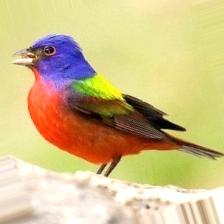
\includegraphics[width=0.24\textwidth]{aug1.jpeg}
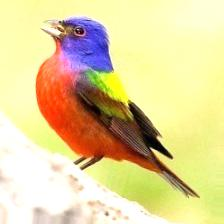
\includegraphics[width=0.24\textwidth]{aug2.jpeg}
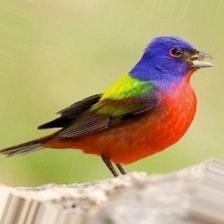
\includegraphics[width=0.24\textwidth]{aug3.jpeg}
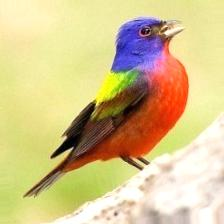
\includegraphics[width=0.24\textwidth]{aug4.jpeg}
	\caption{Rotation, shearing, flipping and brightness adjustments applied to a picture}
\end{figure}

\end{frame}

\begin{frame}{Fourier Transform}

\begin{figure}[!htb]
	\minipage{0\textwidth}
	\raggedleft
	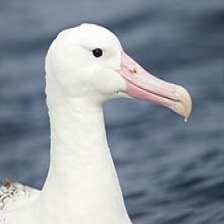
\includegraphics[scale=0.33]{fourier1}
	\endminipage
	\minipage{0.725\textwidth}
	\raggedleft
	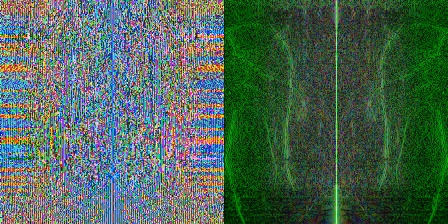
\includegraphics[trim=0cm 0cm 0cm 0cm, scale=0.33]{fourier2}
	\endminipage
	\caption{Left: Original image. Middle: Phase angles. Right: Amplitudes.}
\end{figure}	
\end{frame}

\begin{frame}{Fourier Transform}

\begin{table}[H]
  \caption{Accuracies for the basic CNN}
  \label{sample-table}
  \begin{tabular}{ll}
    Data & Accuracy (\%) \\
    \hline
    Raw Images  & 64.59 \\
    Fourier Angles & 28.84   \\
    Fourier Amplitudes & 48.42 \\
    Fourier Angles \& Amplitueds & 47.42 \\
    \hline
  \end{tabular}
\end{table}

\end{frame}

\begin{frame}{Mixup}

\begin{figure}[h]
	\subfloat{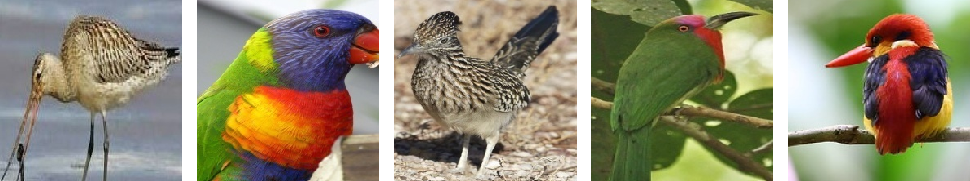
\includegraphics[width=\textwidth]{mixupbirds1.png}} +\\[0.05in]
	\subfloat{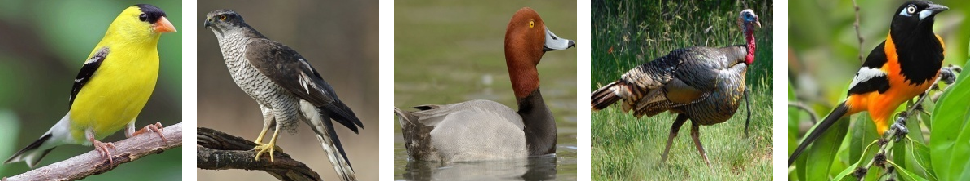
\includegraphics[width=\textwidth]{mixupbirds2.png}} =\\[0.05in]
	\subfloat{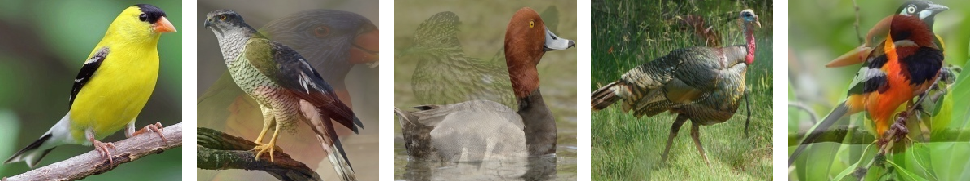
\includegraphics[width=\textwidth]{mixup.png}}
\end{figure}

\end{frame}

\begin{frame}{Mixup}

\begin{figure}[!htb]
	\minipage{0.32\textwidth}
	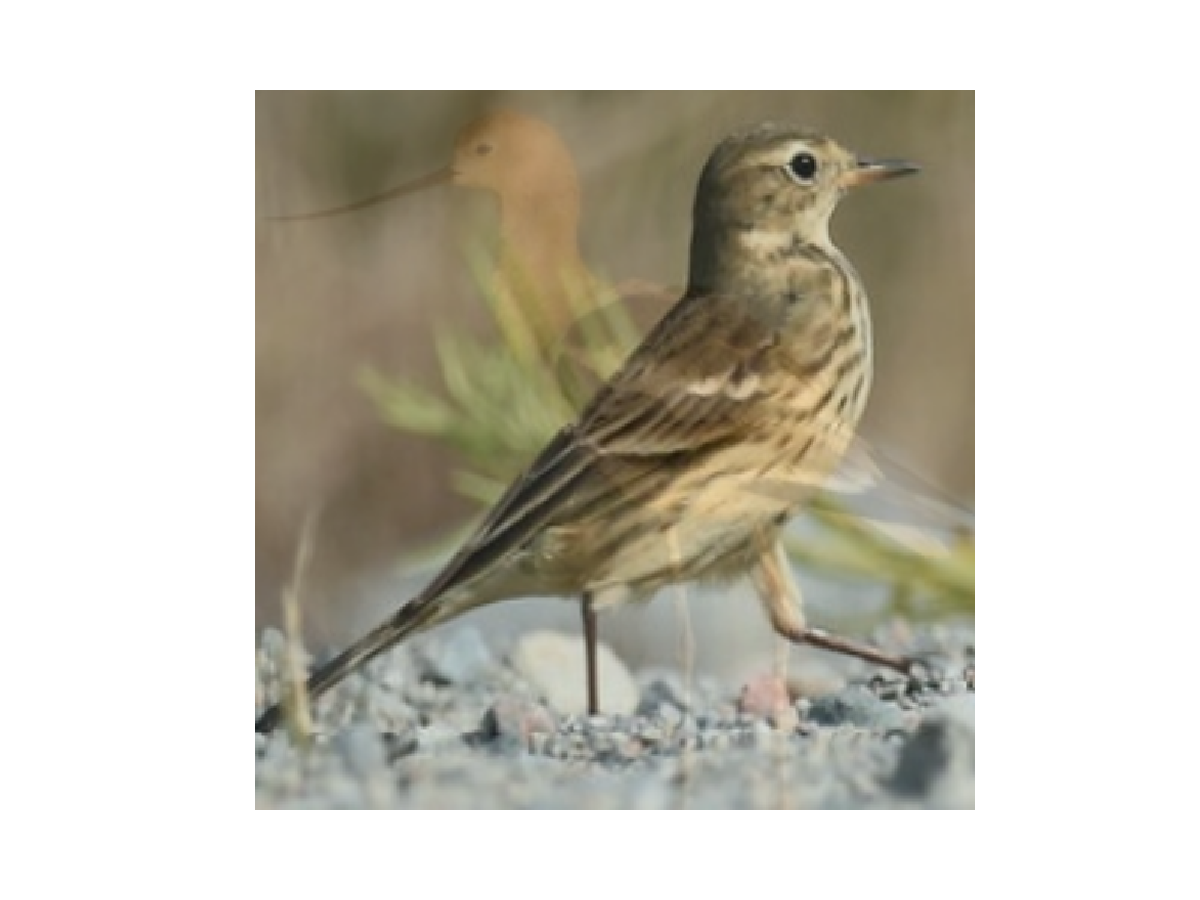
\includegraphics[trim=3cm 2cm 3cm 3cm, width=\linewidth]{mixup1.pdf}
	\endminipage\hfill
	\minipage{0.32\textwidth}
	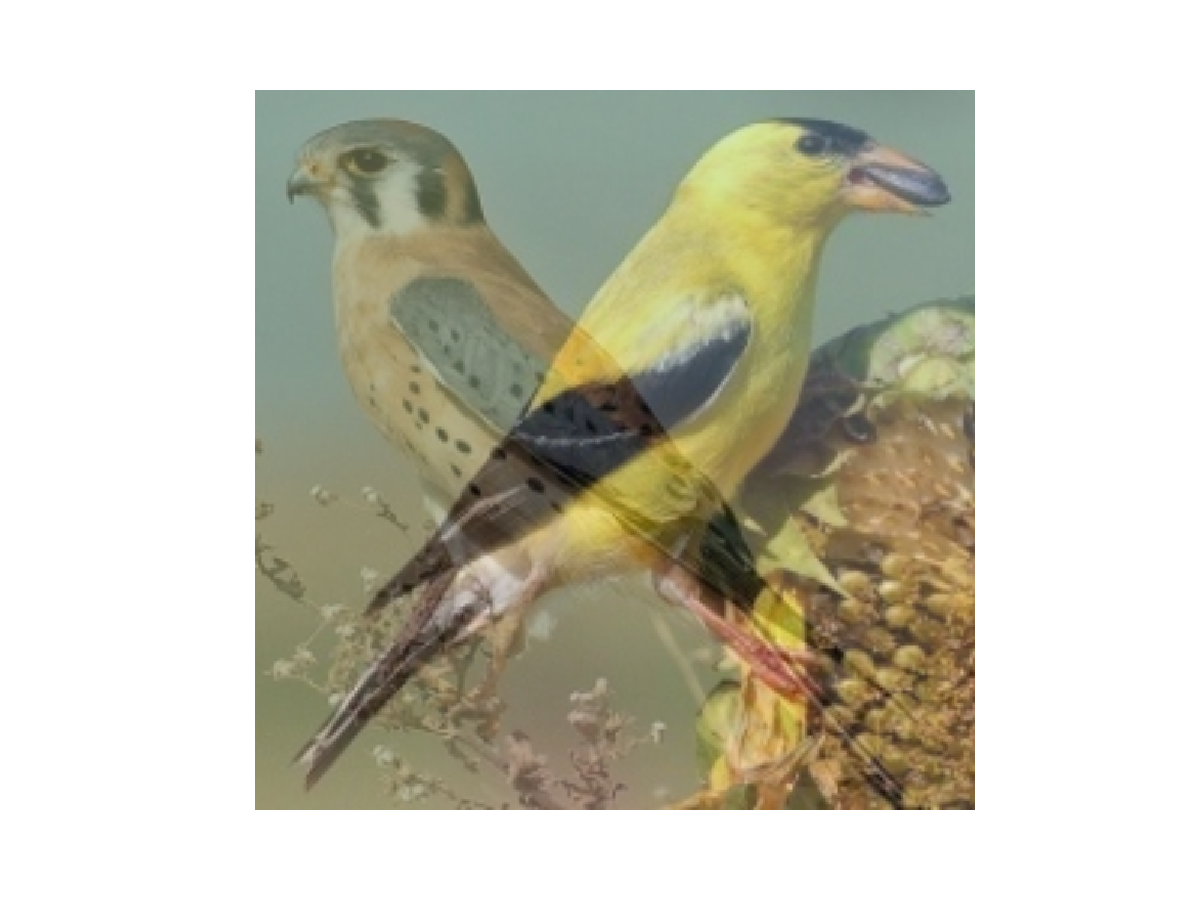
\includegraphics[trim=3cm 2cm 3cm 3cm, width=\linewidth]{mixup2.pdf}
	\endminipage\hfill
	\minipage{0.32\textwidth}%
	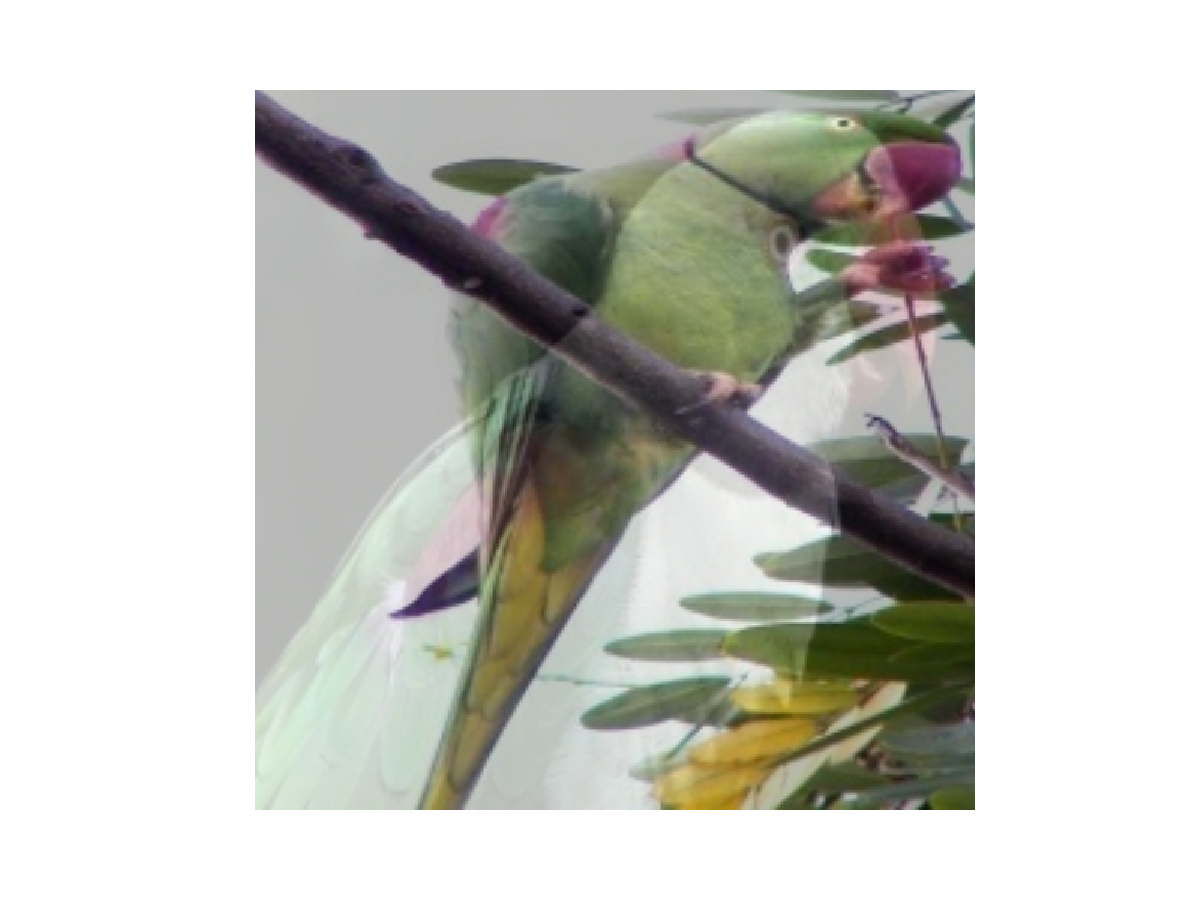
\includegraphics[trim=3cm 2cm 3cm 3cm, width=\linewidth]{mixup3.pdf}
	\endminipage
	\caption{Three examples of mixup performed om images of different bird species.}
\end{figure}

\end{frame}

\begin{frame}{Mixup}

Mixup performances on different networks (for best set of parameters)

\end{frame}

\end{document}